\chapter{Software e tecnologia}

\pagestyle{fancy}

O conceito clássico de um SIG é o de uma aplicação completa que implementa ferramentas para realizar tarefas essenciais com dados geográficos: criação ou edição, manipulação e análise. Com o tempo, surgiram outras formas de aplicações que também se enquadram no âmbito dos SIG.

Neste capítulo, veremos as características dos aplicativos SIG, divididos em três grupos principais: ferramentas de desktop, cartografia na Web (\emph{Web mapping}) e SIG móvel. Também abordaremos aspectos tecnológicos relacionados.

\section{Ferramentas de desktop}

As funções básicas de um SIG de desktop podem ser divididas em cinco blocos: \textbf{entrada e saída de dados, visualização, edição, análise e geração de cartografia}. Um aplicativo de desktop geralmente possui todas essas funcionalidades, embora nem sempre com o mesmo nível de implementação.

\subsection{Entrada e saída de dados}

Um SIG de desktop deve ter capacidade para \textbf{ler} e, opcionalmente, \textbf{gravar dados}. A gravação é essencial quando o SIG permite gerar novas camadas. Em aplicações sem edição ou análise, essa funcionalidade pode não ser necessária.

Graças a bibliotecas e componentes de acesso a dados, os SIG de desktop podem lidar com \textbf{diversos formatos de dados}, ampliando sua \textbf{conectividade}.

Além de arquivos locais, é cada vez mais comum o acesso a \textbf{bancos de dados} e \textbf{serviços remotos}, que veremos adiante neste capítulo.

\subsection{Visualização}

Visualizar dados é uma função central dos SIG — essencial para interpretação, edição e análise. O ambiente visual se baseia em um \textbf{quadro de visualização} (ou canvas) no qual o usuário organiza camadas e ajusta a \textbf{simbologia} (forma de representação).

A ordem das camadas define a \textbf{hierarquia visual}. Ferramentas de navegação (zoom, pan) permitem explorar a visualização (Figura~\ref{Fig:Herramientas_navegacion}).

\begin{figure}[!hbt]
\centering
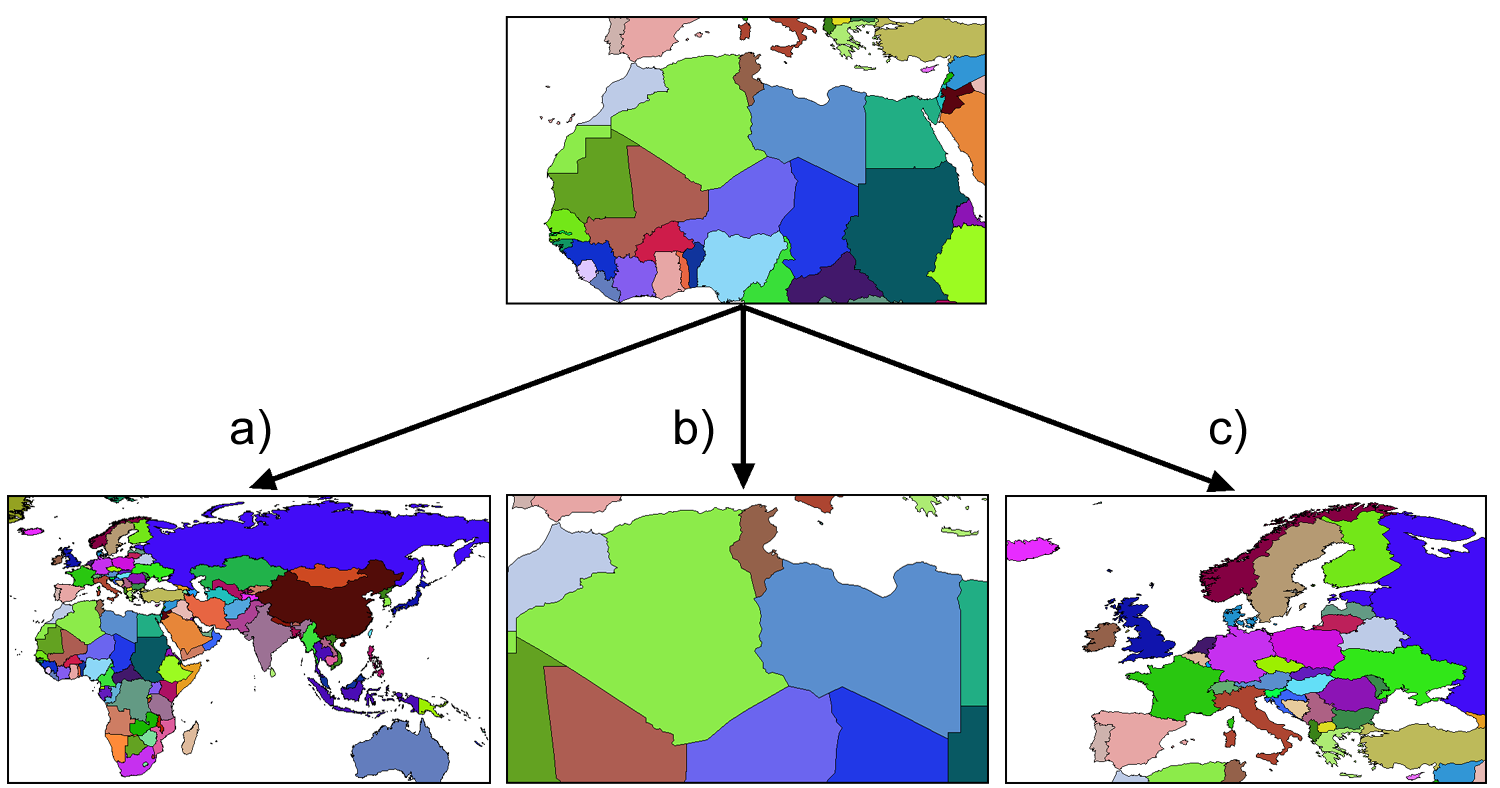
\includegraphics[width=.99\textwidth]{Software/Herramientas_navegacion.png}
\caption{\small Ferramentas básicas de navegação em um SIG de desktop: a) zoom out, b) zoom in, c) deslocamento (pan).}
\label{Fig:Herramientas_navegacion} 
\end{figure}

Diferente de mapas impressos, no SIG o usuário escolhe o que e como visualizar. Dados espaciais são \textbf{independentes de sua simbologia}, e podem ser representados de várias formas — especialmente vetoriais e ráster não visuais.

SIGs também podem ter \textbf{visualização tridimensional}, com controles adicionais para perspectiva, ângulos e relevo.

\subsection{Análise}

Desde o início dos SIG, a \textbf{análise} é uma das funções mais importantes.

Hoje, ferramentas de análise são vistas como \textbf{módulos} sobre uma plataforma base. Elas funcionam de forma \textbf{independente}, mas podem ser combinadas em fluxos de trabalho mais complexos.

Em análises interativas, o usuário interage com o visualizador (por exemplo, clicando num ponto) para fornecer parâmetros.

Na ausência de interação, os módulos funcionam como \textbf{processos automáticos} que recebem dados e retornam um resultado.

SIGs modernos permitem a \textbf{automação} de tarefas complexas por meio de \textbf{modelos de geoprocessamento}, combinando várias etapas em um fluxo.

Além disso, muitos SIG oferecem acesso via \emph{linguagens de script}, o que permite automatizar rotinas e personalizar análises mais sofisticadas.

\subsection{Edição}

Dados geográficos podem ser \textbf{modificados ou atualizados}. A edição é uma funcionalidade essencial em SIGs de desktop.

Podemos editar:

\begin{itemize}
 \item Geometrias vetoriais
 \item Atributos vetoriais
 \item Valores em camadas ráster
\end{itemize}

Ferramentas de edição são inspiradas em softwares CAD. Em alguns casos, também há suporte à edição com \textbf{topologia}.

\subsection{Geração de cartografia}

SIGs de desktop permitem \textbf{gerar mapas para impressão}, com controle sobre layout, legendas, escalas e outros elementos gráficos.

Eles incluem ferramentas para \textbf{automação cartográfica}, como modelos de impressão e geração de séries de mapas (Figura~\ref{Fig:Serie_mapas}).

\begin{figure}[!hbt]
\centering
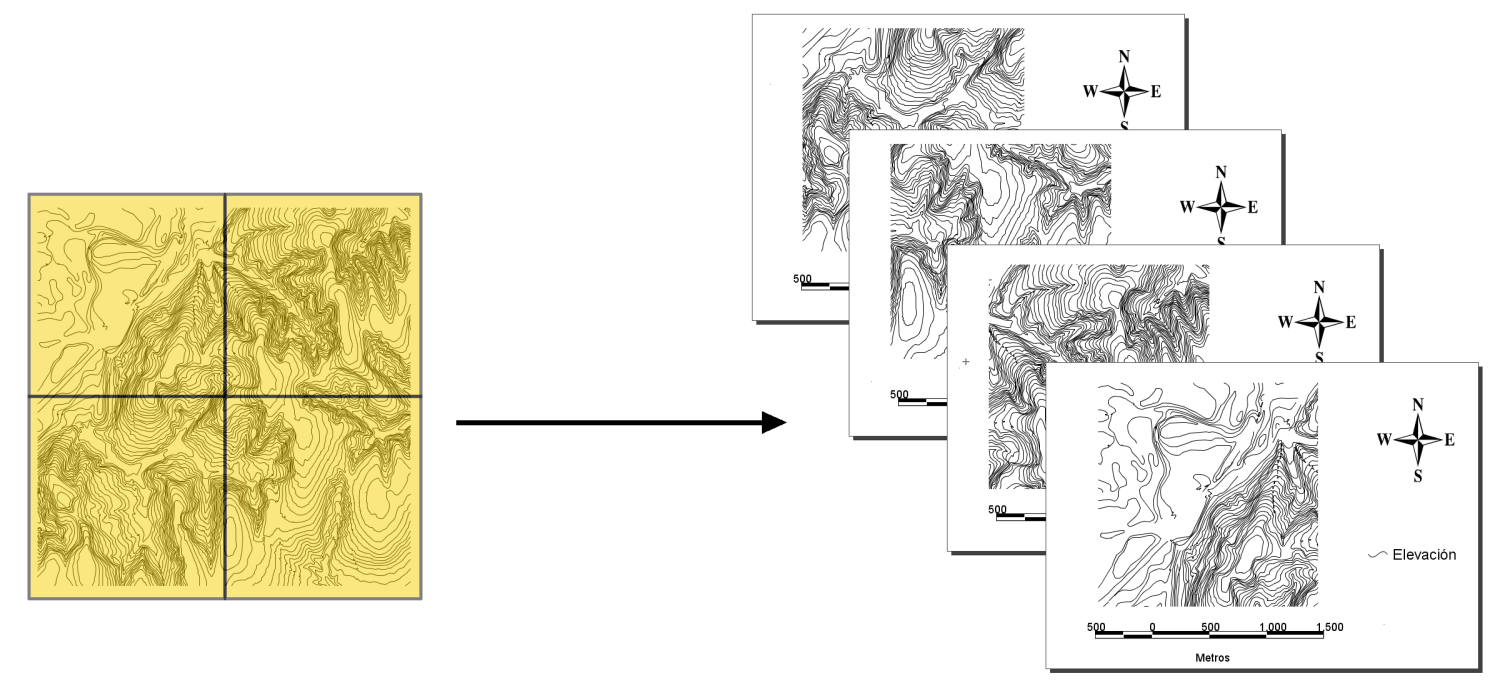
\includegraphics[width=\textwidth]{Software/Serie_mapas.png}
\caption{\small Automação de mapas: divisão de uma área em múltiplas páginas.}
\label{Fig:Serie_mapas} 
\end{figure}

Essa automação é possível porque os dados espaciais são \textbf{separados do design do mapa}.

\section{Cartografia na Web (\emph{Web Mapping}): clientes e servidores}

O \emph{Web Mapping} trouxe os SIG para o ambiente Web. Usa o navegador como plataforma e se baseia na \textbf{arquitetura cliente–servidor}.

O \textbf{servidor} armazena e fornece os dados. O \textbf{cliente} (navegador, app etc.) solicita e usa esses dados.

Exemplo de endereço Web:

\begin{center}
\small\texttt{http://victorolaya.com/writing}
\end{center}

Estrutura:

\begin{itemize}
 \item \texttt{http} — protocolo
 \item \texttt{victorolaya.com} — servidor
 \item \texttt{writing} — recurso (página)
\end{itemize}

Funcionamento básico:

\begin{enumerate}
 \item Cliente faz a requisição
 \item Ela é enviada pela rede até o servidor
 \item O servidor retorna os dados (ou erro)
 \item O cliente renderiza o resultado
\end{enumerate}

Ver Figura~\ref{Fig:Asi_funciona_internet}.

\begin{figure}[!hbt]   
\centering
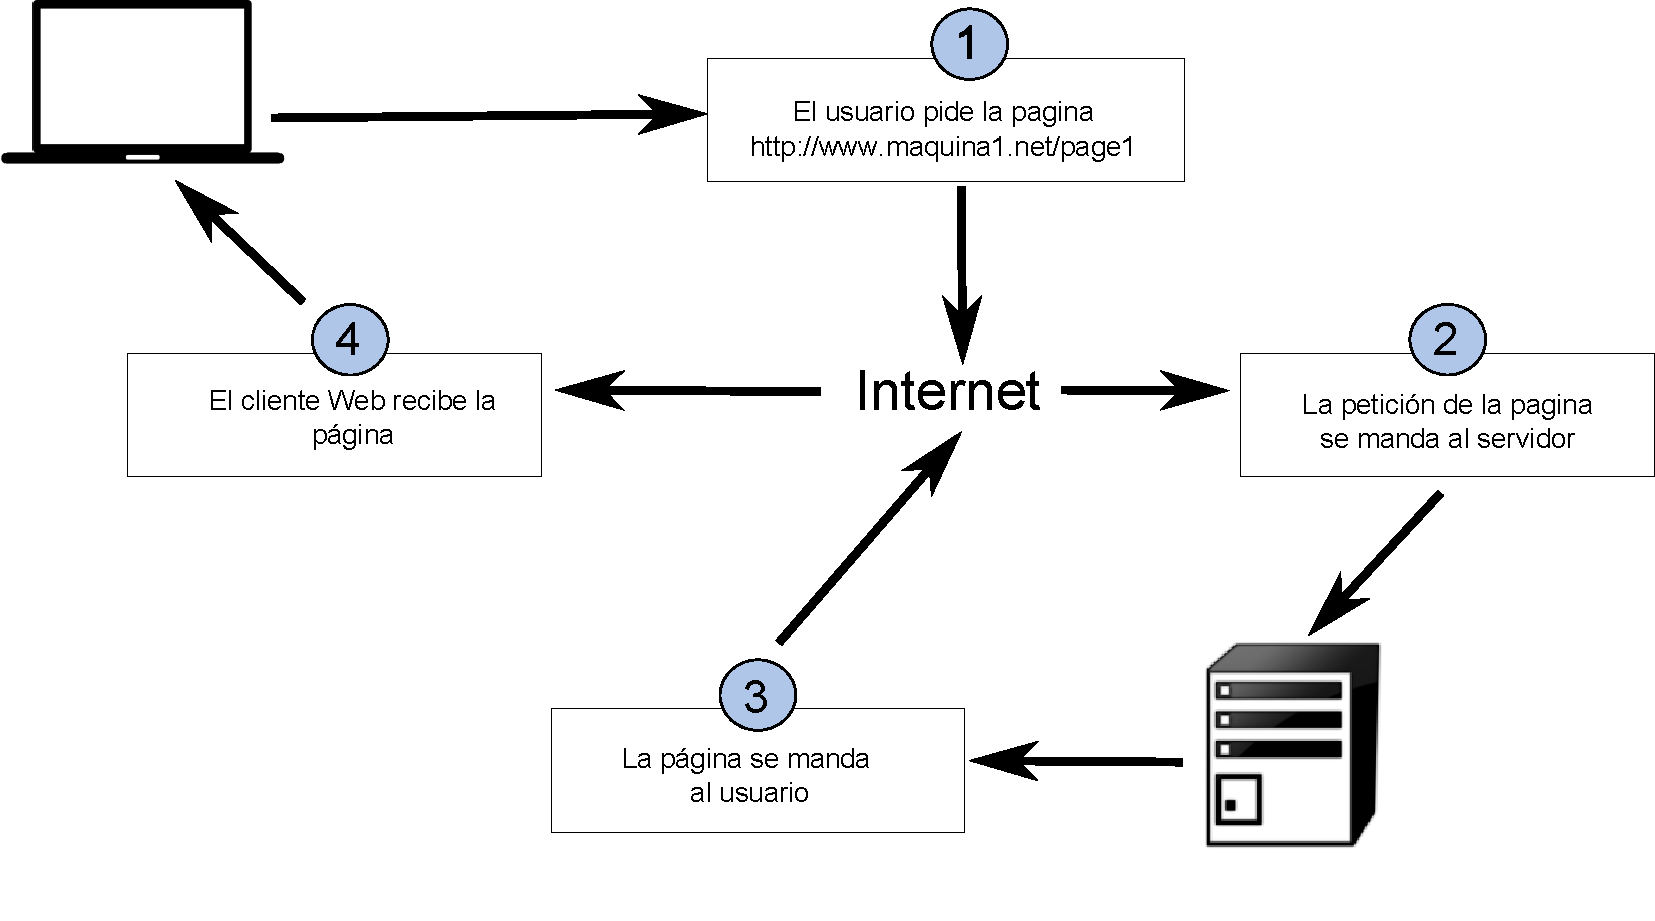
\includegraphics[width=\columnwidth]{Software/Asi_funciona_internet.pdf}
\caption{\small Funcionamento da Web: cliente e servidor.}
\label{Fig:Asi_funciona_internet} 
\end{figure}

Serviços SIG baseados em servidor:

\begin{itemize}
 \item \textbf{Representações gráficas}: imagens geradas pelo servidor
 \item \textbf{Dados brutos}: o cliente recebe os dados e faz a representação ou análise
 \item \textbf{Consultas}: o cliente faz perguntas, e o servidor responde com subconjuntos ou metadados
 \item \textbf{Processos remotos}: o servidor executa análises ou cálculos e retorna os resultados (ver Figura~\ref{Fig:Datos_y_procesos_remotos})
\end{itemize}

\begin{figure}[!hbt]   
\centering
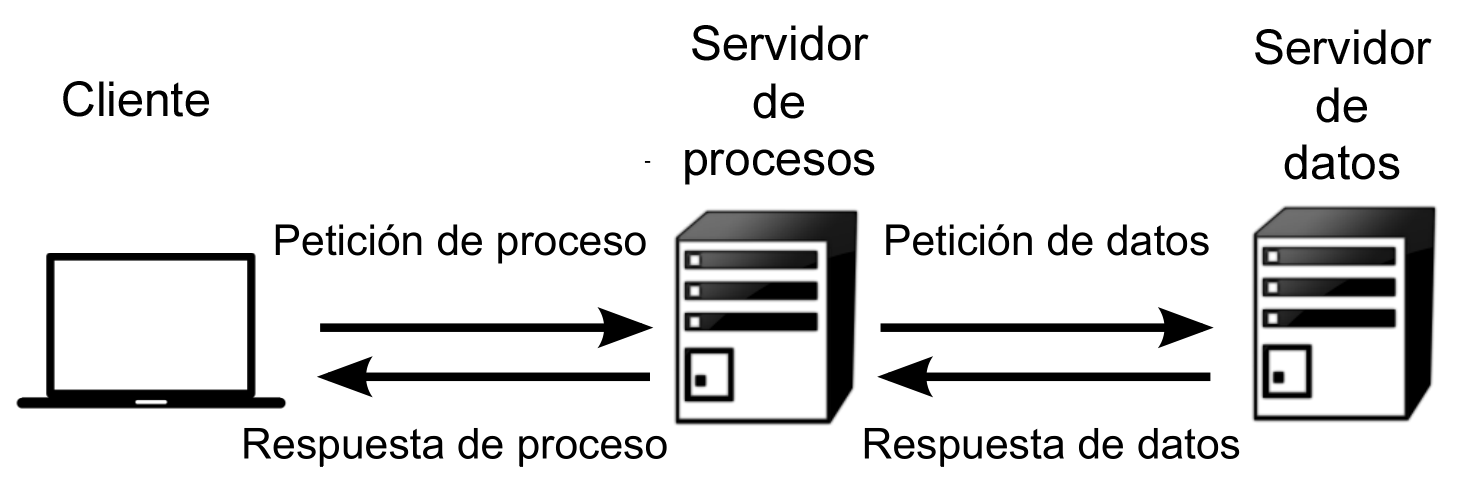
\includegraphics[width=0.95\textwidth]{Software/Datos_y_procesos_remotos.png}
\caption{\small Processamento remoto com acesso a dados em outros servidores.}
\label{Fig:Datos_y_procesos_remotos} 
\end{figure}

Tipos de clientes:

\begin{itemize}
 \item \textbf{Cliente pesado}: software completo (ex: SIG de desktop)
 \item \textbf{Cliente leve}: Web mapping em navegador; simples, mas cada vez mais avançado
\end{itemize}

SIGs Web mais modernos oferecem funcionalidades como edição de camadas, análise e acesso a serviços — formando o chamado \textbf{Web GIS}.

\section{Técnicas para serviços SIG: \emph{Tiling} e \emph{Cache}}

\index{Tiling}\index{Cache}

Essas técnicas são aplicadas principalmente em clientes Web que usam imagens.

\begin{itemize}
 \item \textbf{Tiling}: divide a imagem em mosaicos menores (teselas), otimizando o carregamento
 \item \textbf{Cache}: armazena localmente as teselas já carregadas, evitando downloads repetidos
\end{itemize}

Ver Figura~\ref{Fig:Tiling} para exemplo de economia de dados ao movimentar o mapa.

\begin{figure}[!hbt]   
\centering
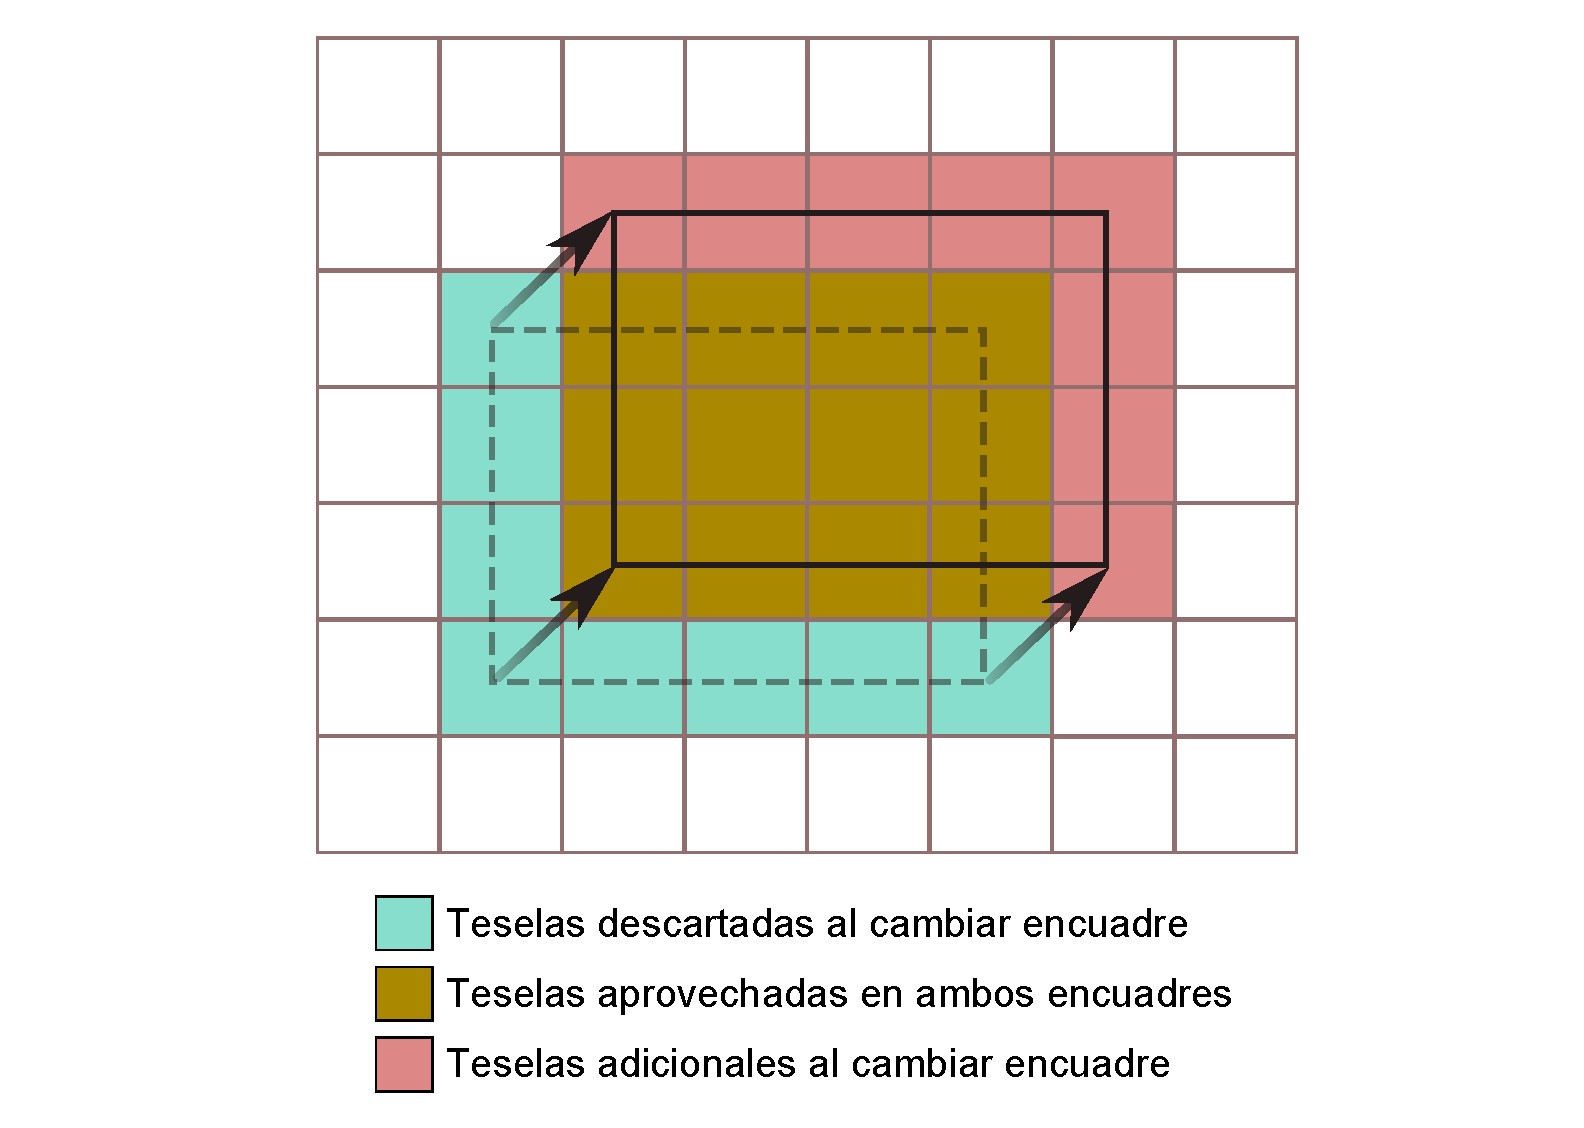
\includegraphics[width=\textwidth]{Software/Tiling.pdf}
\caption{\small Uso combinado de \emph{tiling} e \emph{cache} em um cliente SIG Web.}
\label{Fig:Tiling} 
\end{figure}

Outra técnica recente: \textbf{tiling vetorial}, onde:

\begin{itemize}
 \item Envia-se apenas os dados vetoriais da região visível
 \item O cliente aplica a simbologia localmente
\end{itemize}

Vantagens:

\begin{itemize}
 \item Menor volume de dados
 \item Transições suaves ao mudar de escala
\end{itemize}

\section{Padrões}

Para funcionar corretamente, o sistema cliente–servidor precisa de \textbf{padrões abertos} que garantam \textbf{interoperabilidade}.

Padrões garantem que diferentes sistemas possam se comunicar mesmo se desenvolvidos por fornecedores distintos.

Tipos:

\begin{itemize}
 \item \textbf{De fato} — aceitos na prática
 \item \textbf{De jure} — formalizados por instituições (ex: ISO)
 \item \textbf{Abertos} — disponíveis publicamente, gratuitos e neutros
\end{itemize}

Ver Figura~\ref{Fig:Esquema_no_interoperable} (sem padrões) e Figura~\ref{Fig:Esquema_interoperable} (com padrões).

\begin{figure}[!hbt]   
\centering
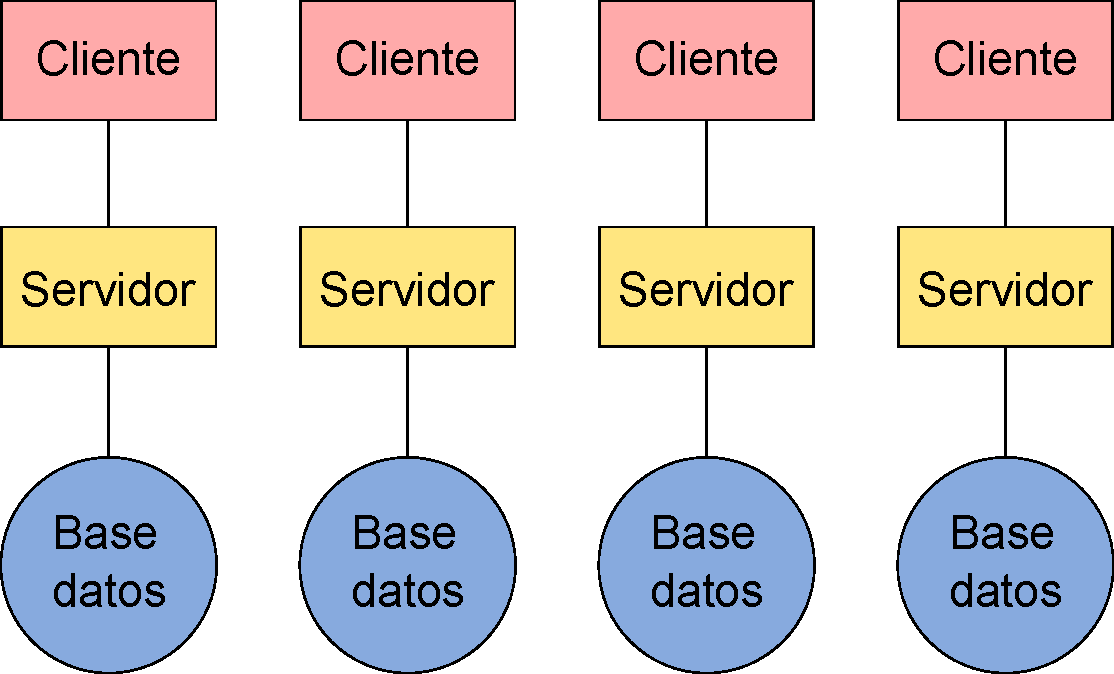
\includegraphics[width=.7\columnwidth]{Software/Esquema_no_interoperable.pdf}
\caption{\small Arquitetura não interoperável.}
\label{Fig:Esquema_no_interoperable} 
\end{figure}

\begin{figure}[!hbt]   
\centering
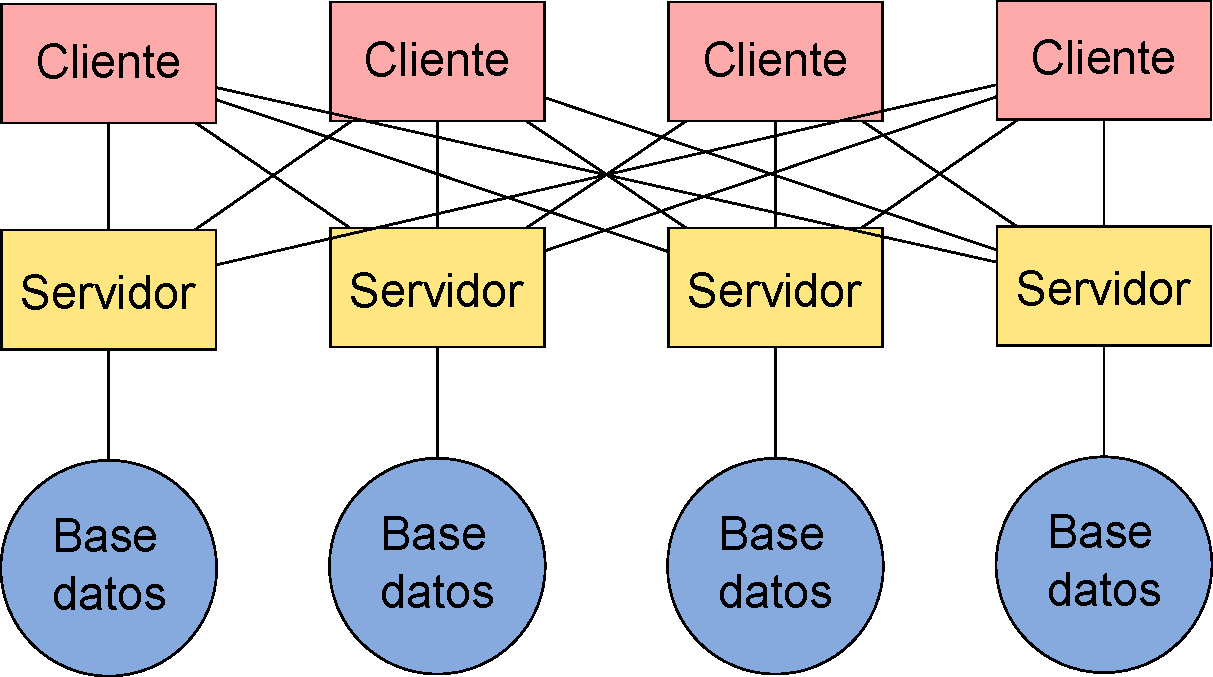
\includegraphics[width=.7\columnwidth]{Software/Esquema_interoperable.pdf}
\caption{\small Arquitetura interoperável baseada em padrões abertos.}
\label{Fig:Esquema_interoperable} 
\end{figure}

Desvantagens da falta de interoperabilidade:

\begin{itemize}
 \item Redundância de dados e alto custo
 \item Múltiplos clientes necessários
 \item Dados e funcionalidades não podem ser combinados
\end{itemize}

\subsection{Principais padrões}

Desenvolvidos pelo \textbf{Open Geospatial Consortium (OGC)}:

\begin{itemize}
 \item \textbf{WMS}: imagens de mapas
 \item \textbf{WCS}: camadas ráster
 \item \textbf{WFS}: camadas vetoriais
 \item \textbf{WPS}: serviços de processamento
 \item \textbf{GML}: formato para armazenamento
 \item \textbf{CSW}: consulta em catálogos
\end{itemize}

Outros padrões relevantes:

\begin{itemize}
 \item \textbf{ISO}: formatos e metadados
 \item \textbf{W3C}: comunicação na Web
\end{itemize}

\section{SIG móvel}

SIGs móveis (celulares, tablets) combinam elementos do SIG tradicional com as funcionalidades dos dispositivos móveis.

Funcionalidades principais:

\begin{itemize}
 \item \textbf{Acesso à Internet}
 \item \textbf{Posicionamento} (manual, via rede ou GPS)
\end{itemize}

Mesmo com limitações, SIGs móveis possibilitam:

\begin{itemize}
 \item \textbf{Coleta de dados em campo}
 \item \textbf{Navegação baseada em localização}
 \item \textbf{Serviços contextuais}
\end{itemize}

Aplicações:

\begin{itemize}
 \item \textbf{Navegação}
 \item \textbf{Inventário geográfico}
 \item \textbf{Guias e informações locais}
 \item \textbf{Publicidade geolocalizada}
 \item \textbf{Monitoramento de pessoas ou objetos}
 \item \textbf{Gestão de ativos ou frotas}
\end{itemize}

Sensores embutidos (GPS, bússola, acelerômetro, luz etc.) expandem as possibilidades do SIG móvel.

\pagestyle{empty}
